\chapter{Contexte : un besoin d'explicabilité}
\paragraph{}Expliquer les modèles de décisions boites noires est un besoin se faisant de plus en plus ressentir et suscitant de nombreux débats et tables rondes dans la communauté scientifique. Les entreprises recherchent avant toute chose la performance et ce au détriment de la transparence des algorithmes utilisés. En effet dans le domaine du machine learning il existe une multitude d'algorithmes pouvant être utilisés afin de fournir une prédiction, mais il existe une corrélation non négligeable entre les performances et la transparence de notre modèle comme le montre la figure \ref{performanceAndInterpretabilite}. En général, plus notre modèle est performant, plus il est difficile à comprendre.

\begin{figure}[h]
\centering
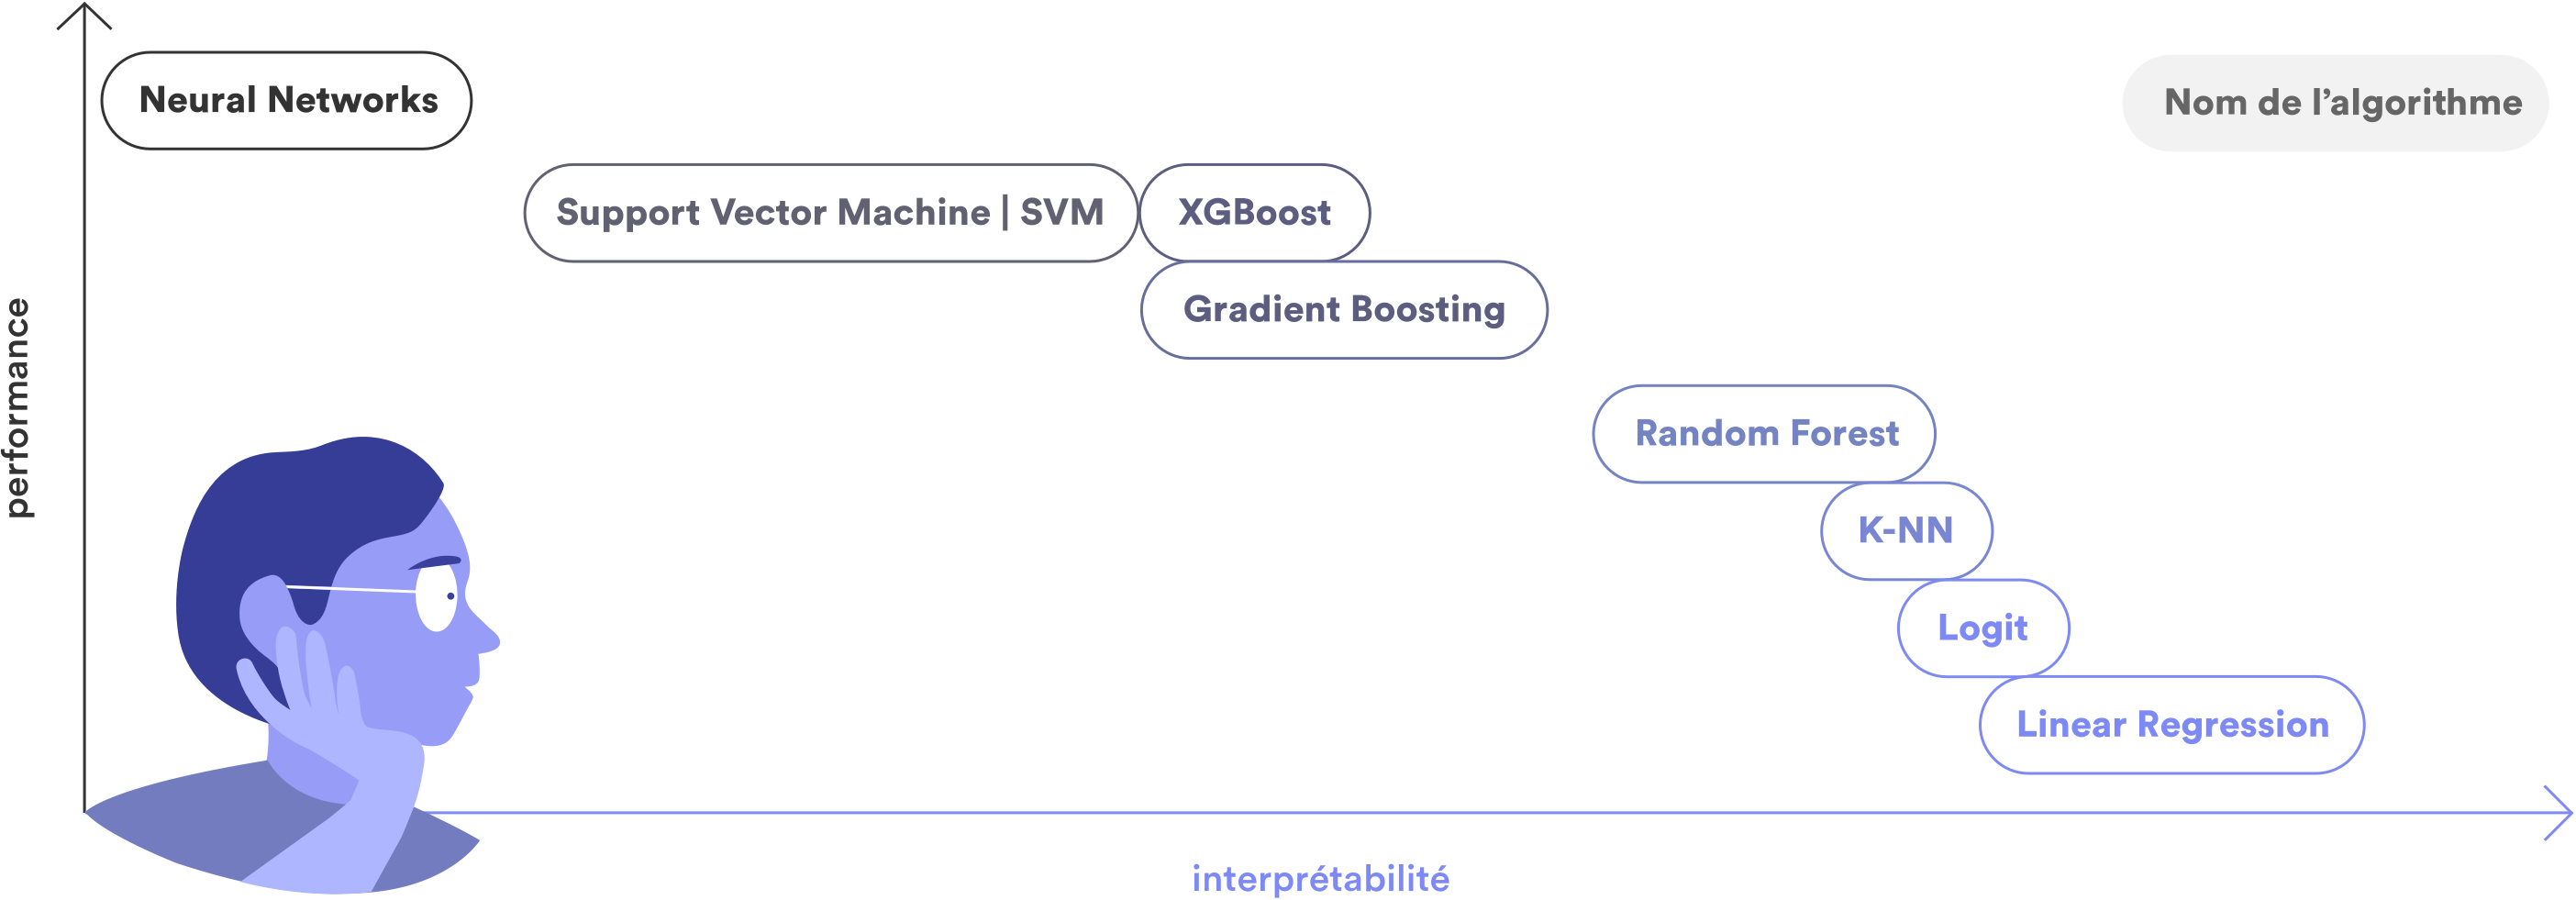
\includegraphics[scale=0.15]{src_img/performanceAndInterpretabilite.png}
\caption{Lien entre la performance et l'interprétabilité d'un algorithme de machine learning. \textit{Source \cite{hippocrate}}}
\label{performanceAndInterpretabilite}
\end{figure}

\paragraph{}À l'heure actuelle, le réseau de neurones artificiels fait partie des algorithmes les plus performante et est le plus couramment utilisée.
La non-explicabilité de ces modèles posent des problèmes de fiabilité, d'éthique et de responsabilité. Ce floue accentue aussi la méfiance et la peur des personnes envers l'intelligence artificielle, et entraîne un problème de compréhension entre les Data Scientist et les experts métier qui en plus de ne pas comprendre comment fonctionne le modèle ne comprennent pas non plus les raisons de son résultat. Aussi, expliquer ces modèles permettrait d'améliorer notre conformité à la loi (notamment vis-à-vis de la RGPD évoqué en introduction) ainsi que d'augmenter les performances de nos modèles. Cette nouvelle problématique présente donc de nombreux enjeux de tailles.

\paragraph{}Ce besoin d'explicabilité se fait tellement ressentir qu'il devient un enjeu de taille même pour les plus hautes instances de l'état. Ainsi, en 2017, le Premier Ministre Français Édouard Philippe confit au mathématicien et député Cédric Villani une mission parlementaire d’information sur la stratégie française et européenne à adopter en matière d'intelligence artificielle. Communément appelé "Rapport Villani" \cite{rapportVillani}, il consacre toute une partie sur les questions d'éthique et arrive au constat suivant : le principal problème vient du fait que l'IA est une boîte noire. L'explicabilité de l'IA est un aspect fondamental de ce rapport et Villani donne des pistes pour améliorer ce domaine :
\begin{itemize}
    \item \textbf{L’audit des IA} : Villani propose \textit{"La constitution d’un corps d’experts dotés des compétences requises semble nécessaire pour procéder à des audits d’algorithmes et de bases de données sur pièce, et procéder à des tests par tout moyen requis."} L'idée est donc d'effectuer des contrôles dans les entreprises afin de palier à toutes dérives.
    \item \textbf{L’évaluation citoyenne des IA} : L'idée est la même que la précédente, mais appuis le fait que le contrôle, en plus d'être mis en place par un organe public, doit aussi provenir de la société civile.
    \item \textbf{Soutenir la recherche sur l’explicabilité} : L'IA et son explicabilité étant des disciplines récentes, le gouvernement se doit d'investir dans la recherche et de favoriser une collaboration étroite entre pouvoirs publics, laboratoires de recherche et industriels.
\end{itemize}

\section{Impact social de l'intelligence artificielle}

\paragraph{}Dans son livre "Weapons of Math Destruction" \cite{mathDestruction} l'américaine Cathy O'Neil qui a une formation en mathématiques, a été trader, puis data scientist dénonce l'impact social engendré par l'utilisation permanente des modèles prédictifs dans nos vies. Le sous-titre de ce livre, qui en résume le propos, est "Comment le big-date augmente les inégalités et menace la démocratie". Pour commencer, Cathy O'Neil souligne le fait qu'un modèle prédictif ne peut pas couvrir la complexité du vrai monde, que les modèles se basent sur des comportements passés et classent les individus en tribus de façon arbitraire alors que la réalité est beaucoup plus complexe. De ce fait, le risque d'erreur est important et les probabilités ne reflètent pas forcément la réalité. Un autre problème est que les jeux de données utilisés ne sont pas nécessairement fiables ou adaptés au modèle et que ces modèles reflètent les choix subjectifs de leurs concepteurs. Le dernier problème majeur soulevé est que ces modèles sont opaques et qu'il n'est pas possible, contrairement au jugement humain, de faire appel en cas de désaccord. En outre, il est possible de camoufler des choix subjectifs (jugements raciaux ou discriminatoires par exemple) en créent un modèle émettant les prédictions allant dans le sens voulu afin de dédouaner la responsabilité sur le modèle.

\paragraph{}L'intelligence artificielle aurait donc pour effet de renforcer le déterminisme social et ainsi d'augmenter les inégalités. Là encore, expliquer ces décisions permettrait de prévenir des potentiels dérives et rendre l'explication obligatoire, dans certains cas, permettrait de remettre la responsabilité sur les concepteurs de ces modèles.

\section{L'éthique}
\paragraph{}De nombreux cas très exposés dans les médias nous montrent que l'incompréhension à l'égard de l'IA peut amener à des problèmes du point de vue éthique. La question de l'éthique est souvent ramenée à deux aspects principaux : la discrimination et la protection des données privées des usagers.

\subsection{La discrimination}
\paragraph{}La question essentielle à se poser est de savoir comment une intelligence artificielle est amenée à prendre des décisions discriminantes. Dans un article, Barocas et Selbst distinguent cinq façons par lesquelles une intelligence artificielle pourrait aboutir à une discrimination \cite{discriminationWay}. Ces cas sont uniquement des cas involontaires et ne prennent pas en compte une discrimination délibérée qui pourrait bien évidemment être possible.
\begin{itemize}
    \item \textbf{Définition des variables cibles et des étiquettes de classes} : le but d'une intelligence artificielle est de découvrir des corrélations dans des jeux de données. Ainsi, certain choix de variables cibles ou d'étiquettes de classes peuvent amener à faire des corrélations discriminatoires. Un exemple trivial serait de considérer un modèle permettant de savoir si un employé fait du travail de qualité, l'entreprise choisira de prendre en compte les retards des employés dans son modèle d'évaluation. Les personnes défavorisées habitant souvent loin de leur lieu de travail, ont plus souvent tendance à être en retard à cause des embouteillages et des problèmes de transport. Ces employés habitant loin, seront jugés comme faisant du travail de moins bonne qualité ce qui n'est pas forcément le cas. Si on ajoute à cela le fait que les personnes issues de l'immigration sont en moyenne plus pauvres et habitent en moyenne plus loin des centres villes, nous pouvons arriver involontairement à une IA discriminante par le simple fait d'utiliser l'étiquette "retard" dans l'évaluation des performances d'un employé.
    \item \textbf{Les données d'apprentissage} : les données d'apprentissage peuvent contenir des biais qui seront ensuite appris par notre modèle. L'exemple de l'IA de recrutement de l'entreprise Amazon qui rejetait les CVs contenant le mot "femme"\cite{amazonAi} évoqué en introduction le montre bien. Cette IA avait en faite appris en analysant tous les profils recrutés par Amzon dans le passé, or les personnes recrutées étaient dans l'ensemble majoritairement des hommes et très majoritairement pour les postes technique. L'IA a donc déduis qu'il était préférable de recruter des hommes.
    \item \textbf{La collecte des données d'apprentissages} : Les lieux dans lesquels sont récoltés les données d'apprentissage sont aussi déterminant. Par exemple si l'on récolte des données concernant la criminalité dans un quartier avec des personnes issues majoritairement de l'immigration, l'IA aura plus tendance à considérer les immigrés comme de potentiels criminels par rapport aux personnes non-imigrées et inversement si on choisit un quartier avec des personnes majoritairement non-imigrées.
    \item \textbf{La sélection des caractéristiques} : Afin que l'IA puisse s'entraîner, il faut lui fournir des données qui sont en réalité une représentation simplifiée de notre monde. Ainsi, son créateur doit faire des choix pour sélectionner les caractéristiques qui constitueront cette représentation. Ce choix peut par concours de circonstance involontairement découler sur de la discrimination il faut donc les choisir avec parcimonie.
    \item \textbf{Données indirect} : Certaines données peuvent inclure des données indirect. Par exemple : \textit{"un jeu de données qui ne contient pas de données explicites sur l’orientation sexuelle peut tout de même la dévoiler. Une étude de 2009 a montré que les liens d’"amis" sur Facebook révèlent par une méthode de prédiction précise l’orientation sexuelle des utilisateurs.} Entre autre, le pourcentage d’"amis" s’identifiant comme homosexuels serait fortement corrélé avec l’orientation sexuelle de l’utilisateur concerné\cite{dicriminationAlgo}.
\end{itemize}
\paragraph{}Mieux comprendre le fonctionnement de nos algorithmes permettrait donc de mieux se prémunir des discriminations involontaires. Aussi on pourrait prendre en compte l'explication en plus de la prédiction afin de fournir un résultat optimal. Par exemple, aux États-Unis, un algorithme appelé Compas est utilisé par les juges pour évaluer la probabilité pour un prévenu de se faire arrêter à nouveau dans les deux ans à venir. Cet algorithme est beaucoup remis en cause, car il est jugé "non-pertinant" et "discriminatoire" par certaines personnes alors que d'autres ont grandement confiance en lui, deux camps s'affrontent donc. Dans ce cas-là, fournir une explication conjointement à la prédiction permettrait de mettre tout le monde d'accord, ainsi nous pouvons prendre en compte la prévision et déterminer si dans le cas précis elle est issue d'un jugement non-pertinant, discriminatoire ou autre.

\paragraph{}Pour répondre aux problèmes d'éthique, le rapport Villani préconise, en plus de l'explicabilité des décisions, de penser l'éthique dès la conception. Notamment en intégrant ces problématiques dans la formation des ingénieurs et chercheurs en IA, ainsi qu'en instaurant une "étude d’impact sur les discriminations" aux acteurs mettant en oeuvre de tels algorithmes.

\subsection{Protection des données}
\paragraph{}L'apprentissage d'une intelligence artificielle requière un très grand nombre de données, parmi lesquelles peuvent se trouver des données personnelles. L'utilisation d'un modèle pourrait donc aussi nécessiter de fournir des données personnelles afin d'effectuer une prédiction. L'utilisation de ces données jugées critiques est problématique, car des restrictions et des règles de protection en découlent. Tel qu'évoqué dans l'introduction, le RGPD par l'addition de plusieurs de ses articles implique un "droit à l'explication", car des données personnelles de l'utilisateur sont utilisées. Ce droit a été démontré par Seth Flaxman et Bryce Goodman \cite{RGPDexplanRight}, ce qui a donc pour effet d'accentuer le besoin d'explicabilité des modèles de décision boites noires. En effet, pour le moment ce droit est inaccessible par les usagers et les entreprises éprouvent des problèmes de responsabilités. En plus des données personnelles, l'intelligence artificielle met en évidence des angles morts dans la législation actuelle. En effet, de nombreuses données jugé non-personnelles sont collectées et ce sans aucun contrôle car la législation ne prend en compte que les données à caractère personnel. La collecte de nombreuse données jugé non-personnelles pouvant, par corrélation, découler sur des informations personnelles, un flou juridique existe. Mais interdire la collecte de données aurait pour effet d'empêcher le développement de ces nouvelles technologies utiles et prometteuses, la question est donc de définir où mettre le curseur entre la protection des utilisateurs et le développement des technologies. La solution souvent évoquée est l'anonymisation qui consiste à collecter des données personnelles, mais à retirer toutes informations permettant de remonter jusqu'à la personne à qui appartient ces données. La collecte de données est une question épineuse qui sera sûrement amenée à faire évoluer la loi.

\section{Fiabilité et confiance}
\paragraph{}Deuxièmement, expliquer les décisions prisent par un modèle boite noire permettrait d'augmenter la fiabilité que l'on lui accorde. Le modèle peut très bien fonctionner dans la plupart des cas, mais il est possible qu'il réagisse mal dans un certain cas bien spécifique. Avec l'absence de compréhension du fonctionnement interne de notre modèle, nous pouvons ne pas prévoir ce cas spécifique qui représente un risque. Le domaine médical par exemple est en attente d'une plus grande fiabilité de ses modèles en effet, une erreur peut avoir des conséquences graves et mettre en danger des personnes. La manière classique de mesurer la fiabilité d'un modèle est de calculer sa précision (accuracy), cela consiste simplement à diviser le nombre de prédictions corrects par le nombre de prédiction total. Cette méthode indispensable ne permet pas à elle seule de juger la fiabilité de notre modèle, admettons que nous arrivons à une précision de 100\% rien ne nous dis que dans un cas très particulier notre modèle ne nous donnera pas une prédiction fausse. La compréhension de la logique interne de notre modèle serait donc un facteur supplémentaire afin d'appuyer la fiabilité que l'on lui donne.
\paragraph{}De plus, un soudage publié par OpinionWay\cite{opinionWay} montre que 30\% des Français ont peur d'un jugement porté par l'intelligence artificielle dans le domaine financier et 21\% dans le domaine médical. L'incompréhension de la logique interne des algorithmes décisionnels tend à accentuer la méfiance envers ces technologies. Fournir une explication permettrait d'augmenter l'acceptation de ces nouvelles technologies par le grand publique.

\section{Performance}
\paragraph{}Expliquer la logique interne d'un modèle pourrait aussi être utile durant son développement afin de comprendre par exemple pourquoi il ne fonctionne pas bien dans certains cas voir même pourquoi il ne converge pas du tout. Ce qui aurait pour effet de simplifier son développement et améliorer sa compétitivité.

\paragraph{}Mais l'explication a un coût, outre le temps de développement, fournir une explication à chaque prédiction augmenterait le temps nécessaire à la prise de décision. Deux facteurs principaux entrent en jeu, le premier est le temps de calcul, le deuxième est le temps nécessaire à la lecture et à la compréhension de l'explication par un humain. Ainsi, dans certains domaines où la décision doit être prise extrêmement rapidement, fournir une explication ne sera pas possible pour la prise de décision, mais on pourrait imaginer qu'elle puisse être fournit à posteriori afin d'expliquer pourquoi le modèle a pris une telle décision pour des questions de responsabilité par exemple.

\paragraph{}De plus, l'explication n'est pas exempte des prérequis classiques. Elle se doit elle aussi d'être précise, robuste et fiable, ainsi l'explicateur (entité fournissant l'explication) devra être testé et approuvé par des personnes compétentes dans le domaine de la prédiction cible. On pourrait donc l'évaluer et instaurer un seuil minimum de précision par exemple. Un autre aspect important à prendre en compte est la robustesse, on pourrait par exemple se poser les questions suivantes : l'explicateur fournit-il la même explication deux fois de suite pour une même instance ? Pour deux modèles entraînés avec le même code et le même jeu de données, l'explication pour une instance donnée est-elle la même ? L'explicateur est-il sensible aux potentiels bruits blancs (hasard ne pouvant être modélisée) de l'instance ?

\paragraph{}Il est nécessaire de garder en tête  que l'explication est l'interprétation d'un modèle qui interprète le mode réel, nous ne devons pas donner une confiance aveugle à notre explication ni même à notre prédiction sous prétexte qu'elle est fournie avec une explication.
